\documentclass{scrreprt}
\usepackage{etex}
\usepackage[ngerman]{babel}
\usepackage[utf8]{inputenc}
\usepackage[T1]{fontenc}
\usepackage{amsmath, amssymb}
\usepackage{graphicx}

\usepackage{pgfplots}
\pgfplotsset{compat=1.11}
\usepgfplotslibrary{external}
\usepackage{pgfplotstable}

\usepackage{booktabs}
\usepackage{multirow}
\usepackage{longtable}
%\usepackage{ulsy}
%\usepackage{pst-all}
\usepackage{picture}
\usepackage[automark]{scrpage2}
\usepackage{caption}
\pagestyle{scrheadings}
\ihead[]{Friedrich Hübner 2897111}
\ohead[]{Fiona Paulus 2909625} 

\author{Friedrich Hübner 2897111\\
Fiona Paulus 2909625}
\title{Computerphysik\\Hausarbeit 4}

\begin{document}
\maketitle
\newpage

\chapter*{Der Differentialgleichungssolver}
Für den DGL-Solver wird das Runge-Kutta-Verfahren mit den Fehlbergkoeffizienten und automatischer Schrittweitensteuerung aus der Vorlesung verwendet. Die Berechnung aller Werte erfolgt genau nach diesem Verfahren.

\section*{Programm (abgabe4\_runge\_kutta.cpp)}
In dieser Datei befindet sich der DGL-Solver, der von allen anderen Programmen eingebunden wird.\\

Mit der Funktion 'runge\_kutta\_init(f, $t_0$, $y_0$)' wird der DGL-Solver initialisiert. Dabei ist $f: \mathbb{R} \times \mathbb{R}^n \to \mathbb{R}^n$ die Differentialgleichung ($y' = f(t,y)$), $t_0 \in \mathbb{R}$ der Anfangszeitpunkt und $y_0 \in \mathbb{R}^n$ der Anfangswert.\\

Mit der Funktion 'runge\_kutta\_iterate()' wird ein Schritt ausgeführt und die neue optimale Schrittweite berechnet.\\

Außerdem werden in der Datei Operatoren für Vektorarithmetik (+,+=,-,*) und für Ausgabe von Vektoren (<\.<) überladen. Zusätzlich gibt es noch Funktionen für den Betrag von Vektoren und das Skalar- und Kreuzprodukt.  

\chapter*{Aufgabe 1 : Doppelpendel}
\section*{allgemeine Hinweise}
Das Programm wurde unter Linux-Mint mit "g++ -std=c++11 -g -Wall -Wextra -pedantic-errors 1.cpp -o 1.exe"\;kompiliert.
\section*{Aufgabenteil (a)}
Aufstellen der Koordinaten:
\[x_1 = L sin(\phi_1)\]
\[y_1 = 2L - Lcos(\phi_1)\]
\[x_2 = L sin(\phi_1)+ L sin(\phi_2)\]
\[y_2 = 2L - L cos(\phi_1) - L cos(\phi_2)\] 
Daraus ergibt sich die Lagrangefunktion:

\[L(\phi_1,\phi_2,\dot{\phi_1},\dot{\phi_2}) = 1/2 m L^2 (2 \dot{\phi_1}^2 + \dot{\phi_2}^2 + 2 \dot{\phi_1}\dot{\phi_2} cos(\phi_1 - \phi_2)) - m g L(4-2 cos(\phi_1)-cos(\phi_2)\]
Aus dieser werden die verallgemeinerten Impulse berechnet.

\[p_1 = \frac{\partial L}{\partial\phi_1} = m L^2 (2\dot{\phi_1}+\dot{\phi_2} cos(\phi_1 - \phi_2))\] 

\[p_2 = \frac{\partial L}{\partial \phi_2} = m L^2(\dot{\phi_2}+ \dot{\phi_1}cos(\phi_1-\phi_2))\]
Die Hamiltonfunktion setzt sich zusammen aus $\phi_1, \phi_2, \dot{\phi_1}$ und $\dot{\phi_2}$

\[H = \sum_{i=1}^{2} p_i \dot{\phi_i} - L = m L^2 (2 \dot{\phi_1} + \dot{\phi_2} cos(\phi_1-\phi_2)\phi_1 + (\dot{\phi_2}+\dot{\phi} cos(\phi_1 - \phi_2)))\]
Durch einsetzten der Bewegungsgleichungen für $\phi_1$ und $\phi_2$

\[\dot{\phi_1}=\frac{1}{m L^2}\frac{p_1-p_2cos(\phi_1-\phi_2)}{1+sin(\phi_1-\phi_2)^2}\] 	

\[\dot{\phi_2}=\frac{1}{m L^2}\frac{2 p_2 - p_1 cos(\phi_1 - \phi_2)}{1+sin(\phi_1-\phi_2)^2}\]
ergibt sich:

\[H = \frac{1}{m L^2}\frac{p_1^2+p_2^2-2 p_1 p_2 cos(\phi_1-\phi_2)}{1+sin(\phi_1-\phi_2)^2}+m g L (4-2cos(\phi_1)-cos(\phi_2))\]
Und durch partielle Ableitung von H nach $\phi_i$ ergeben sich die Bewegungsgleichungen für $p_1$ und $p_2$:

\[\dot{p_1} = -\frac{1}{m L^2}\frac{p_1 p_2 sin(\phi_1-\phi_2)}{1+sin(\phi_1-\phi_2)^2}+\frac{sin(\phi_1-\phi_2) cos(\phi_1-\phi_2) }{m L^2}\frac{p_1^2+2 p_2^2-2 p_1 p_2 cos(\phi_1-\phi_2)}{(1+sin(\phi_1-\phi_2)^2)^2}\]\[-2 m g L sin(\phi_1)\]

\[\dot{p_2}=\frac{1}{m L^2}\frac{p_1 p_2 sin(\phi_1-\phi_2)}{1+sin(\phi_1-\phi_2)^2}-\frac{sin(\phi_1-\phi_2)cos(\phi_1-\phi_2)}{m L^2}\frac{p_1^2 + 2 p_2^2 - 2 p_1 p_2 cos(\phi_1-\phi_2)}{(1+sin(\phi_1-\phi_2)^2)^2}\]\[- m g L sin(\phi_2)\]

\section*{Aufgabenteil (b)}
Das durch die Hamiltonfunktion aufgestellte System von Bewegungsgleichungen werden numerisch mit dem Runge-Kutta-Verfahren numerisch gelöst.

\section*{Aufgabenteil (c)}
Das in Aufgabenteil (b) geschriebene Progamm wird für die Anfangsbedingungen $\phi_1 = 45^\circ$ und $\phi_2=135^\circ$ sowie $\phi_1=10^\circ$ und $\phi_2=5^\circ$ ausgeführt.\\
Daraus ergeben sich folgende Bahnkurven:
\begin{center}
	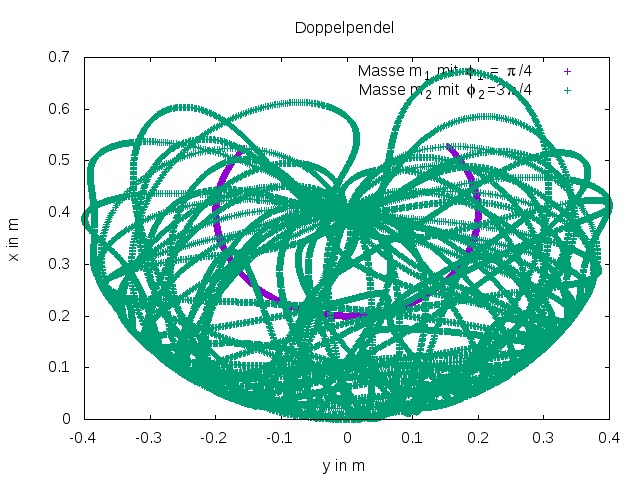
\includegraphics[scale=0.7]{1a.jpeg}
	\captionof{figure}{Bahnkurven der Massen im Doppelpendel für Anfgangsbedingungen\\ $\phi_1=45^\circ$ und $\phi_2=135^\circ$}
\end{center}

\begin{center}
	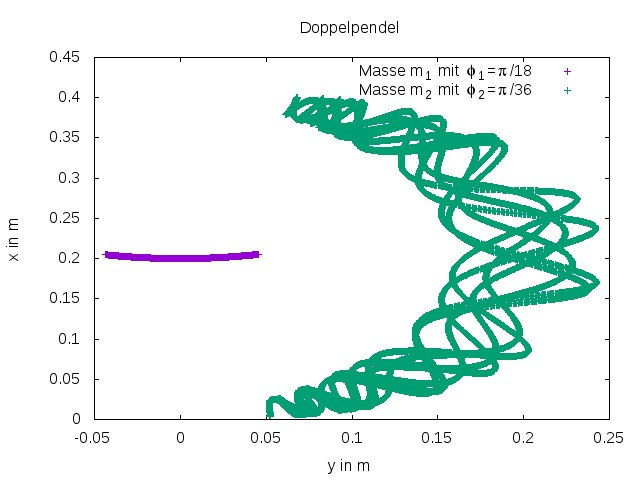
\includegraphics[scale=0.7]{1b.jpeg}
	\captionof{figure}{Bahnkurven der Massen im Doppelpendel für Anfangsbedinugnen \\ $\phi_=10^\circ$ und $\phi_2=5^\circ$}
\end{center}

\section*{Aufgabenteil (d)}
Zur Bestimmung der zeitlichen Entwicklung der relativen Fehler der Hamiltonfunktion wird die Differenz der numerisch gelösten Hamiltonfunktion und des mithilfe der Anfangsbedingungen errechnete Wert in Anhängigkeit von der Zeit geplottet.

\begin{center}
	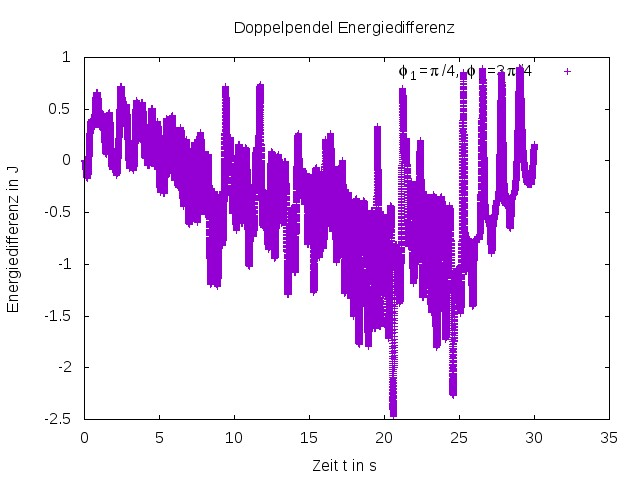
\includegraphics[scale=0.7]{1ae.jpeg}
	\captionof{figure}{zeitliche Entwicklung der Abweichung der Hamiltonfunktion vom wahren Wert $H=1.29 J$ für Anfangsbedinungen $\phi_1=45^\circ$ und $\phi_2=135^\circ$}
\end{center}

\begin{center}
	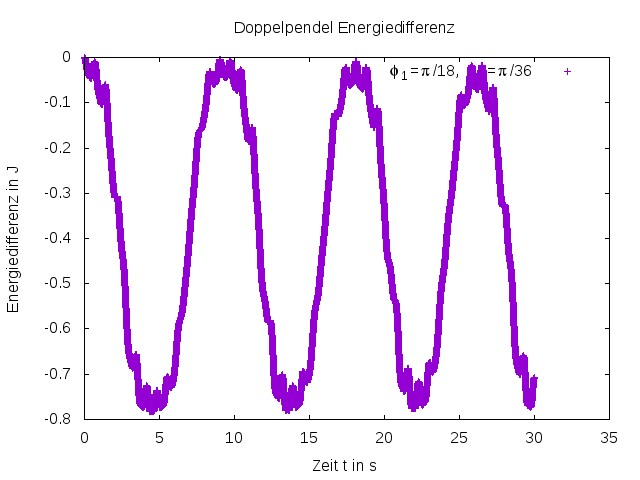
\includegraphics[scale=0.7]{1be.jpg}
	\captionof{figure}{zeitliche Entwicklung der Abweichung der Hamiltonfunktion vom wahren Wert $H=0.41 J$ für Anfgangsbedingungen $\phi_1=10^\circ$ und $\phi_2=5^\circ$}
\end{center}

Aus den Graphen kann man erkennen, dass die Differenz des Anfangswerts der Hamiltonfunktion und der durch Runge-Kutta berechneten Werte in der gleichen Größenordnung liegen und die Abweichung beschränkt ist.

\section*{sonstige abgegebene Dateien}
\subsection*{1.plt}
Die Plot-Datei für die abgegebenen Plots.
\subsection*{1a.txt}
Ausgabedatei des Programms "1.cpp" mit Anfangsbedingungen $\phi_1=45^\circ$,$\phi_2=135^\circ$,$p_1=0$ und $p_2=0$.
\subsection*{1b.txt}
Ausgabedatei des Programms "1.cpp" mit Anfangsbedingungen $\phi_1=10^\circ$,$\phi_2=5^\circ$,$p_1=0$ und $p_2=0$.

\chapter*{Aufgabe 2: Meteorit in der Atmosphäre}
\section*{allgemeine Hinweise}
Das Programm wurde unter Linux-Mint mit "g++ -std=c++11 -g -Wall -Wextra -pedantic-errors 2.cpp -o 2.exe"\;kompiliert.
\section*{Aufgabenteil (a)}
Die Bewegungsgleichung für $\ddot{h}$ ergibt sich aus den Kräften.

\[m_k \ddot{h}=-F_G+F\]
\[m_k \ddot{h}=-G\frac{m_k m_E}{(h+R_E)^2}+ \frac{1}{2}c_W \rho_0 e^{-\frac{M g_0}{R T}h}A \dot{h}^2\]
\[\ddot{h}=-G \frac{m_E}{(h+R_E)^2}+\frac{1}{2 m_k}c_w \rho_0 e^{-\frac{M g_0}{R T}h}A \dot{h}^2\] \\
mit Gravitationskonstante $G=6.67408 \cdot 10^{-11} \frac{m^3}{kg s^2}$, Erdmasse $m_E=5.9722 \cdot 10^{24} kg$, Erdradius $R_E = 6370 \cdot 10^3 m$, $c_W = 0.45$, Dichte am Erdboden $\rho_0 = 1.29 \frac{kg}{m^3}$, mittlerer Molarer Masse $M = 0.02896 \frac{kg}{mol}$, Erdbeschleunignung $9.81 \frac{m}{s^2}$, Gaskonstante $R=8.314 \frac{kg m^2}{s^2 mol K}$ und der Temperatur $T=273 K$.
Die Querschnittsfläche $A$ und die Masse $m_k$ des Kometen berechnen sich durch:

\[A = \frac{\pi}{2}*d^2 = \frac{\pi}{2}(1\cdot 10^{-3})^2 = 1.57 \cdot 10^{-6}\]
\[m_k = \rho_k*V_k = \rho_k * \frac{\pi}{6} d^3 = 7800 \frac{kg}{m^3} \frac{\pi}{6}(1 \cdot 10^{-3})^3 = 4.084 \cdot 10^{-6} \]
mit Dichte des Kometen $\rho_k = 7800 \frac{kg}{m^3}$ und Durchmesser des Kometen $d = 1 \cdot 10^{-3}m$.\\
Durch Umwandlung der Differentialgleichung 2. Ordnung in ein Gleichungssystem 1. Ordnung ergibt sich:
\[\dot{h} = v\]
\[\dot{v} = -G \frac{m_E}{(h+R_E)^2} + \frac{1}{2 m_k}c_w \rho_0 e^{- \frac{M g_0}{R T}h}A v^2\]

\section*{Aufgabenteil (b)}
Die oben aufgestellten Differentialgleichungen werden mithilfe des Runge-Kutta-Verfahrens für verschiedene Anfagsbedingungen numerisch gelöst.
Durch plotten der sich daraus ergebenden Geschwindigkeiten in Abhängigkeit der Höhe ergibt sich folgende Grafik:

\begin{center}
	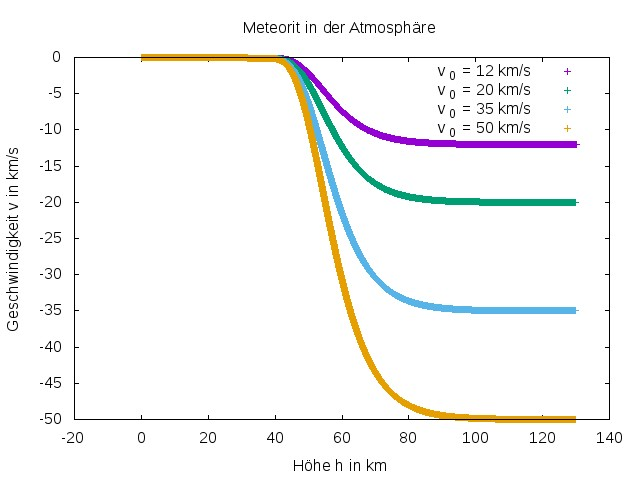
\includegraphics[scale=0.7]{2.jpeg}
	\captionof{figure}{Geschwindigkeiten des Meteorits in Abhängigkeit der Höhe für verschiedene Anfangsgeschwindigkeiten $v_0$}
\end{center}

\section*{sonstige abgegebene Dateien}
\subsection*{2.plt}
Die Plot-Datei für die abgegebenen Plots.
\subsection*{2a.txt}
Ausgabedatei des Programms "2.cpp" mit Anfangsbedingungen $h_0 = 130000 m$ und $v_0 = 12000 \frac{m}{s}$
\subsection*{2b.txt}
Ausgabedatei des Programms "2.cpp" mit Anfangsbedingungen $h_0 = 130000 m$ und $v_0 = 20000 \frac{m}{s}$
\subsection*{2c.txt}
Ausgabedatei des Programms "2.cpp" mit Anfangsbedingungen $h_0 = 130000 m$ und $v_0 = 35000 \frac{m}{s}$
\subsection*{2d.txt}
Ausgabedatei des Programms "2.cpp" mit Anfangsbedingungen $h_0 = 130000 m$ und $v_0 = 50000 \frac{m}{s}$

\chapter*{Aufgabe 3}
\section*{Allgmeine Hinweise}
Das Programm wurde unter Windows 10 mit "g++ -o abgabe4\_3.exe -Wall -Wextra -std=c++0x -O2 -static abgabe4\_3.cpp"\;kompiliert.

\section*{a)}
Die Bewegungsgleichung lautet einfach:
\begin{align}
m\ddot{\vec{x}} &= e\dot{\vec{x}} \times \vec{B}\\
				&= e\dot{\vec{x}} \times \left(\cfrac{\mu_0}{4\pi}\cfrac{3\vec{x}(\vec{x} \cdot \vec{m}) - \vec{m}\cdot\vec{r}^2}{|r|^5}\right)  
\end{align}

Der Dipol wurde Richtung z-Achse gelegt: $\vec{m} = (0,0,m)^T$.\\

Für $\vec{y} = (\vec{x},\dot{\vec{x}})$ gilt nun:\\
\begin{align}
\dot{\vec{y}} = \left(\dot{\vec{x}},  \cfrac{e}{m}\dot{\vec{x}} \times \left(\cfrac{\mu_0}{4\pi}\cfrac{3\vec{x}(\vec{x} \cdot \vec{m}) - \vec{m}\cdot\vec{r}^2}{|r|^5}\right)\right)  
\end{align}

\section*{b) Programm (abgabe4\_3.cpp)}
Das Programm benutzt den Fehlberg-DGL-Solver. Die verwendete Funktion f ist dabei in a) gegeben. Die Anfangsbedingungen muss man in das Programm eintragen. Das Programm simuliert 100s und gibt aller 0.1s Simulationzeit die aktuelle Zeit, Position und Geschwindigkeit aus.  

\section*{c)}
Da der Dipol in z-Richtung angeordnet ist, sind die Feldlinien am Äquator parallel zur z-Achse. Also startet das Proton mit $\vec{v} = (-1000,0,v_z)^T$.
\subsection*{1. $\mathbf{v_z = 100km/s}$}
\subsubsection*{i)}
\begin{center}
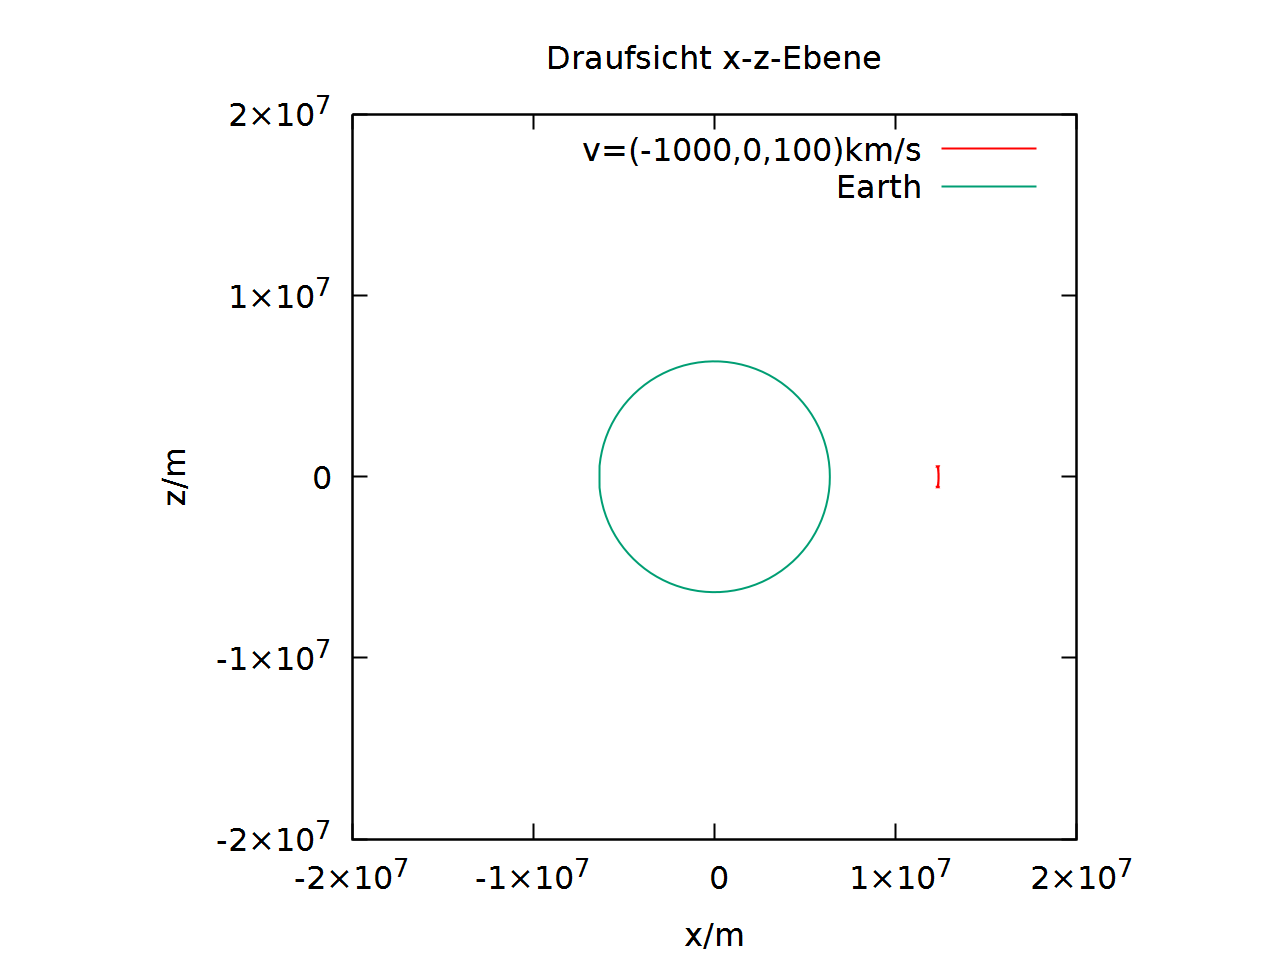
\includegraphics[scale=0.25]{plot_1_i.png}
\end{center}
\subsubsection*{ii)}
\begin{center}
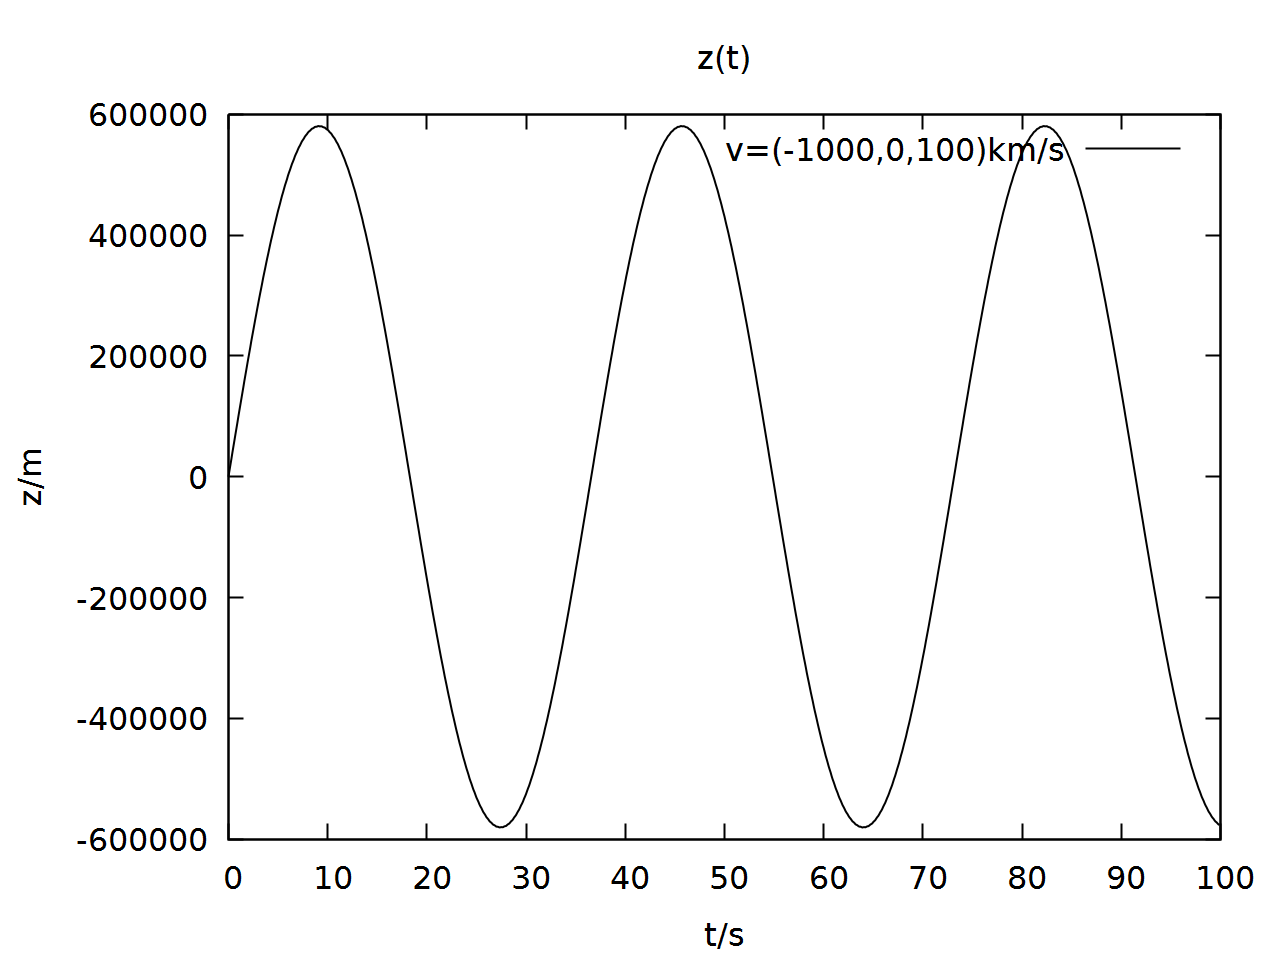
\includegraphics[scale=0.25]{plot_1_ii.png}
\end{center}
\subsubsection*{iii)}
\begin{center}
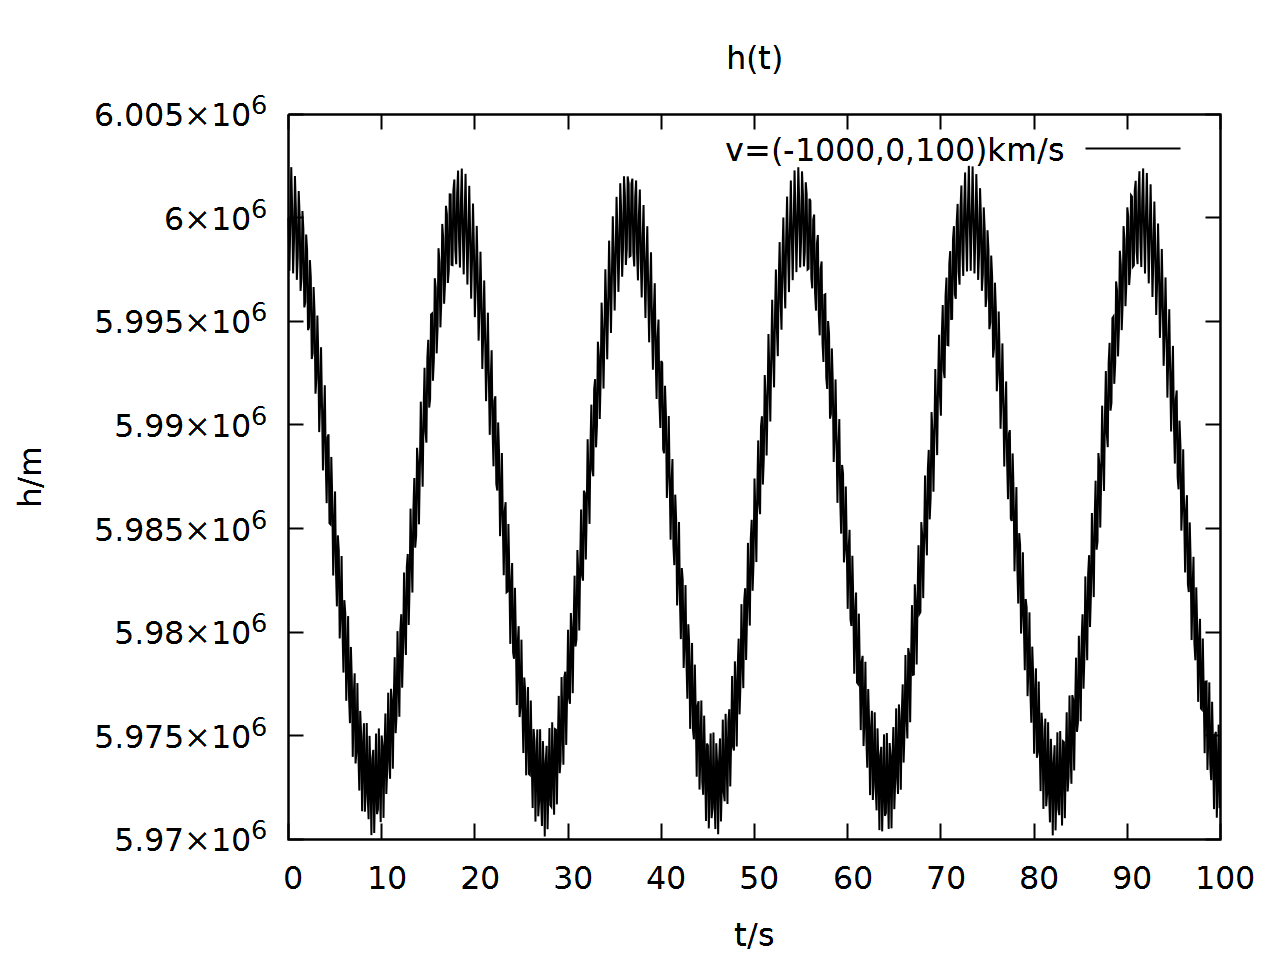
\includegraphics[scale=0.25]{plot_1_iii.png}
\end{center}

\subsection*{2. $\mathbf{v_z = 1000km/s}$}
\subsubsection*{i)}
\begin{center}
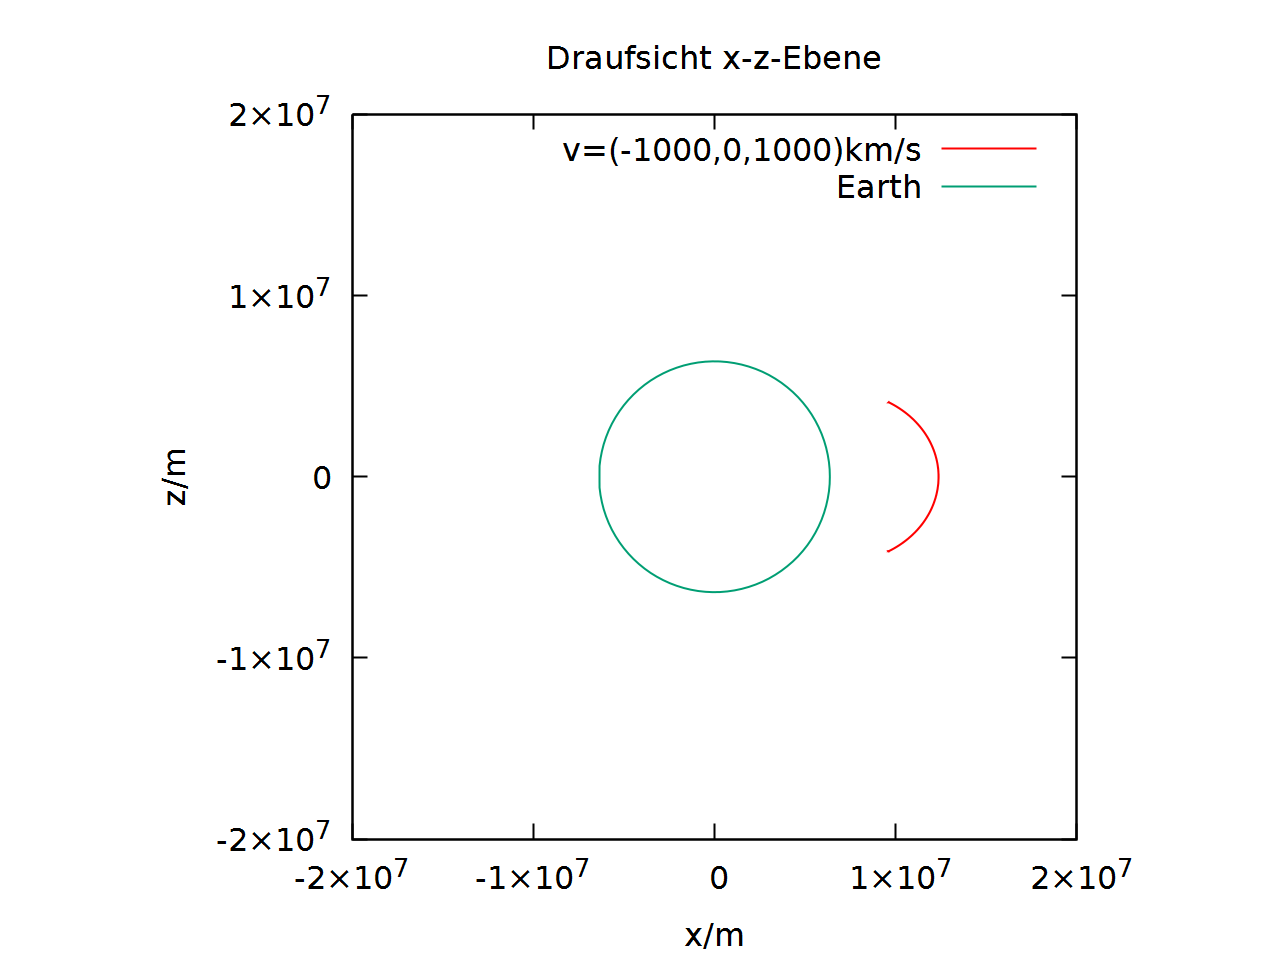
\includegraphics[scale=0.25]{plot_2_i.png}
\end{center}
\subsubsection*{ii)}
\begin{center}
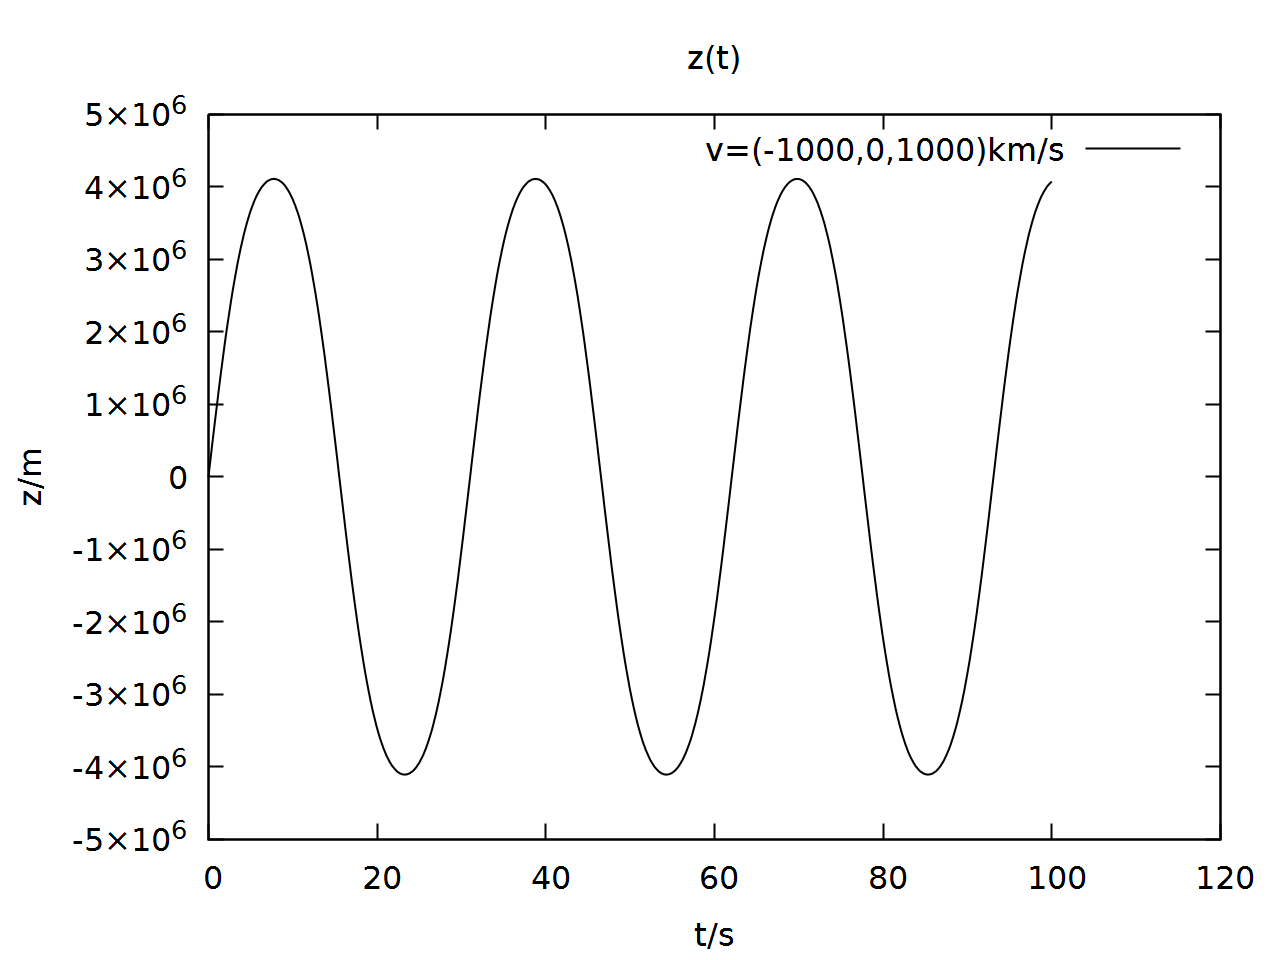
\includegraphics[scale=0.25]{plot_2_ii.png}
\end{center}
\subsubsection*{iii)}
\begin{center}
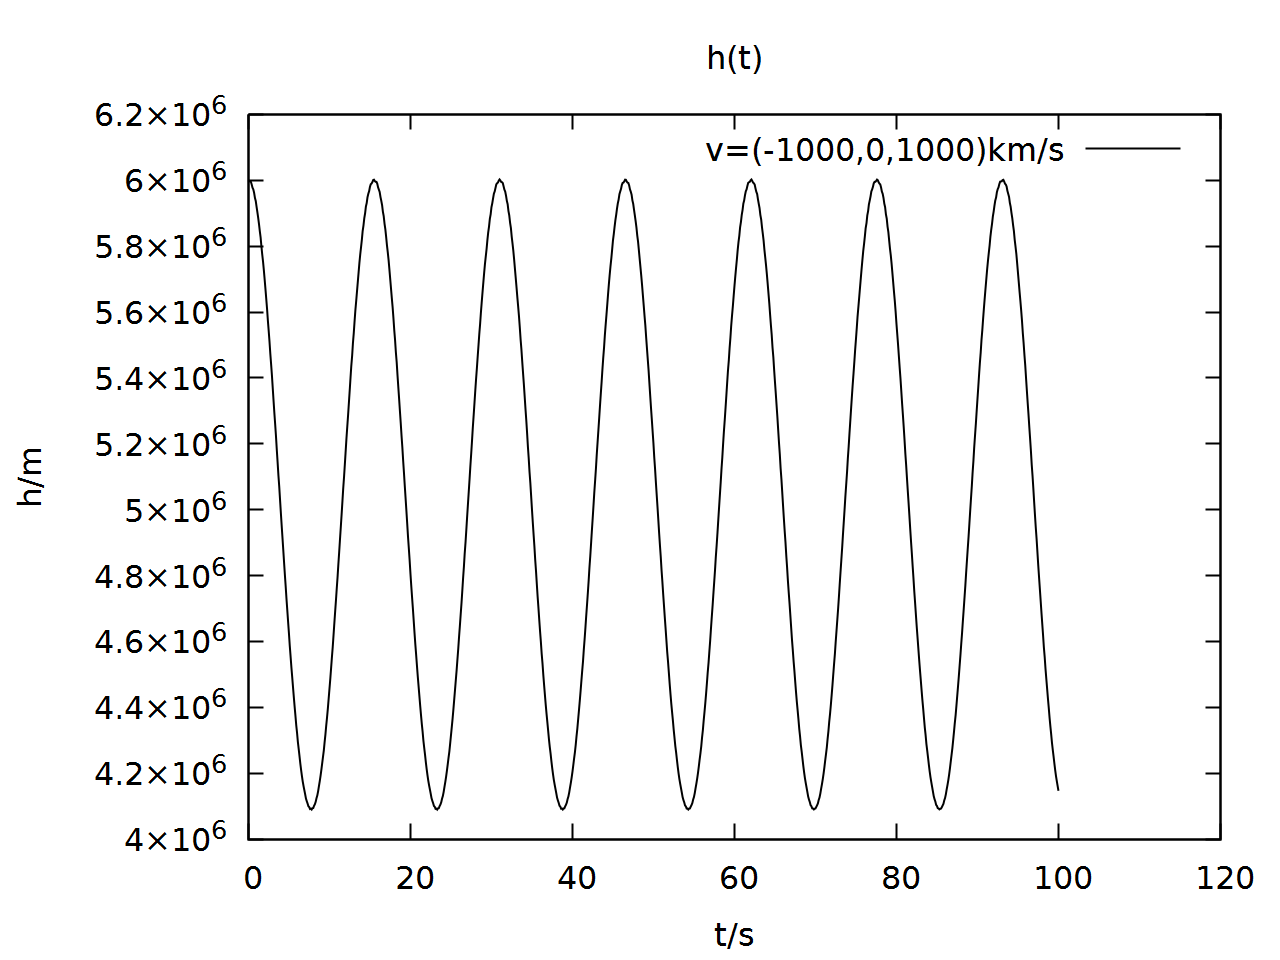
\includegraphics[scale=0.25]{plot_2_iii.png}
\end{center}

\subsection*{3. $\mathbf{v_z = 3000km/s}$}
\subsubsection*{i)}
\begin{center}
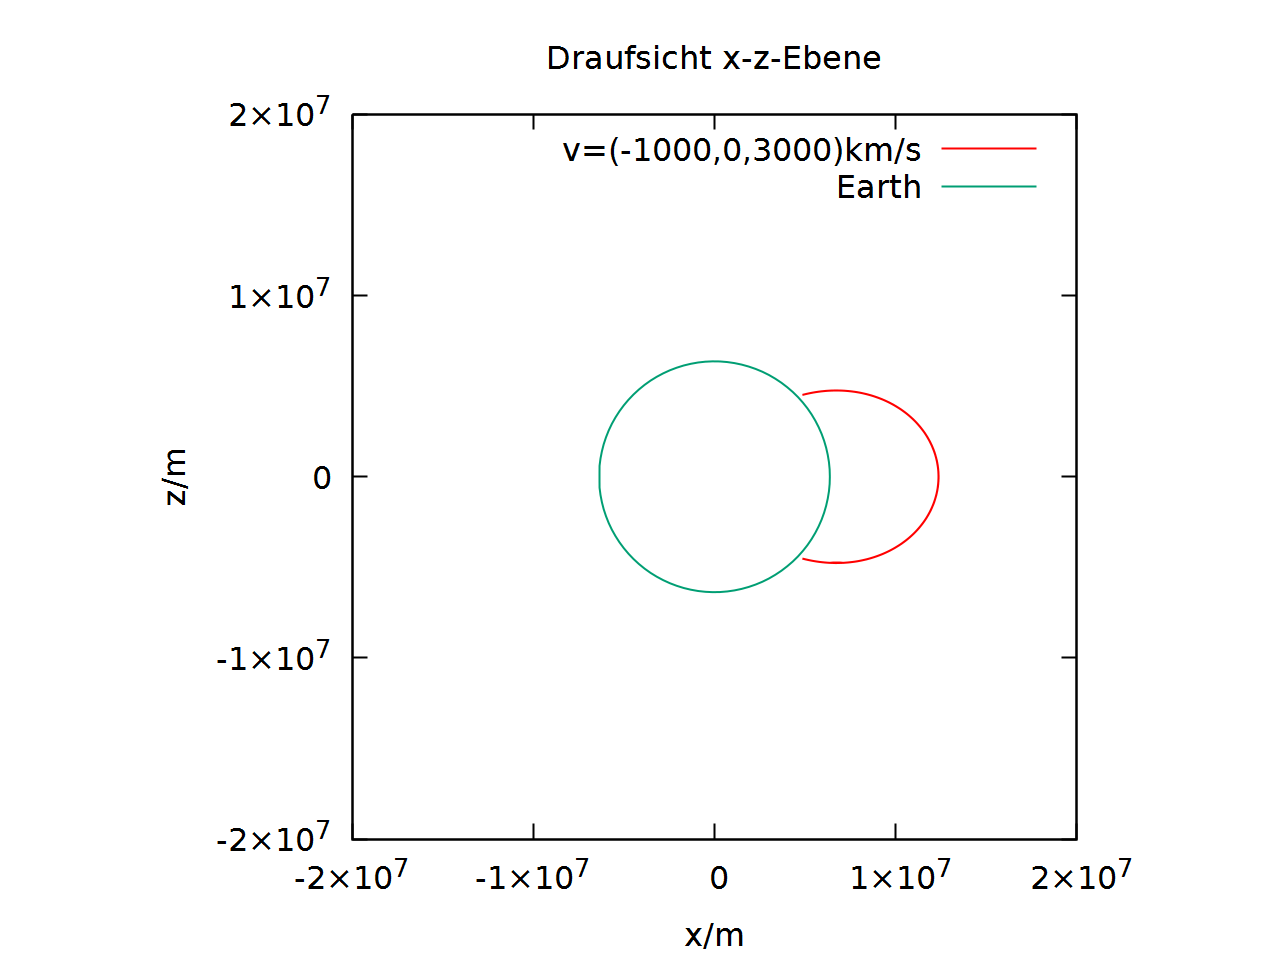
\includegraphics[scale=0.25]{plot_3_i.png}
\end{center}
\subsubsection*{ii)}
\begin{center}
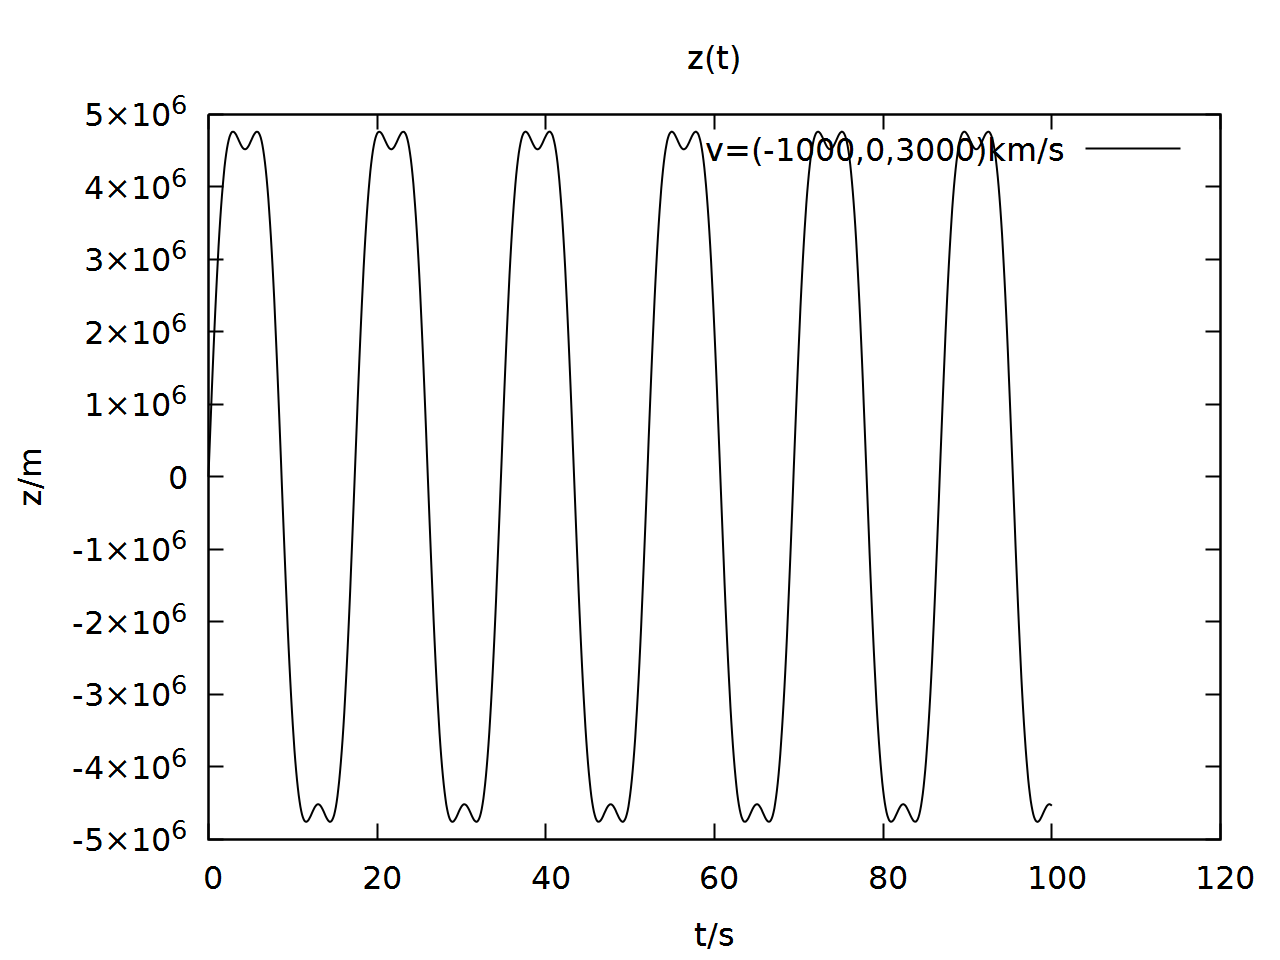
\includegraphics[scale=0.25]{plot_3_ii.png}
\end{center}
\subsubsection*{iii)}
\begin{center}
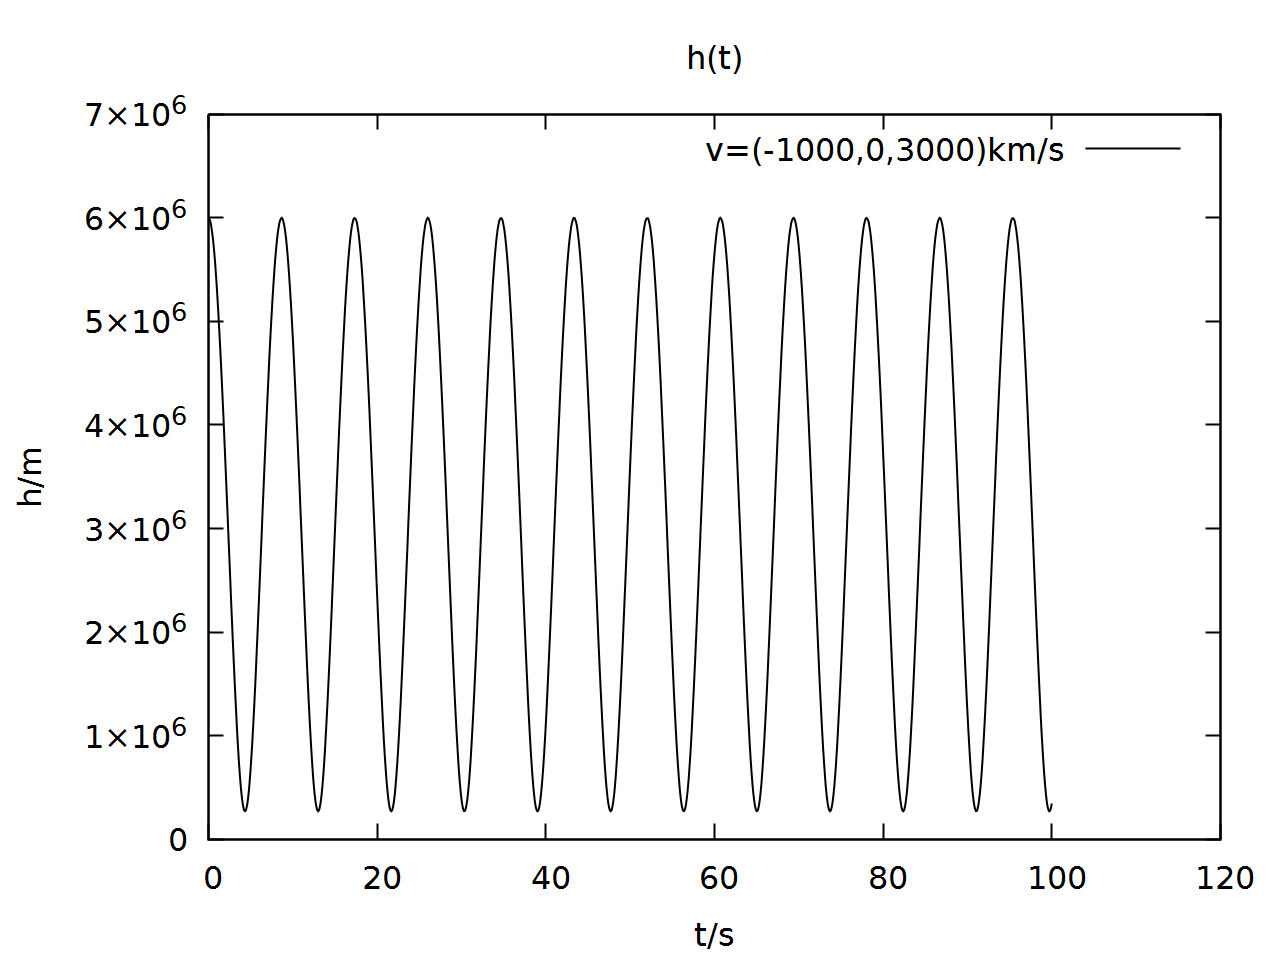
\includegraphics[scale=0.25]{plot_3_iii.png}
\end{center}



\section*{Sonstige abgegebene Dateien}
\subsection*{plot\_i.plt, plot\_ii.plt, plot\_iii.plt}
Die Plot-Dateien für die Diagramme für jeweils Fall i), ii), iii)
\subsection*{1.txt, 2.txt, 3.txt}
Die Ausgabedateien für die einzelnen Anfangswerte
\end{document}